\documentclass[12pt]{article}
\usepackage[latin1,utf8]{inputenc}
\usepackage[brazil]{babel}
\usepackage{setspace}
\usepackage{boxedminipage}
\usepackage{latexsym}
\usepackage{multirow}
\usepackage[pdftex]{graphicx}
\usepackage{float}
\usepackage{url}
\usepackage{xcolor,listings}
\usepackage{amsmath,mathrsfs}
\usepackage{biblatex}
\usepackage[portuguese, ruled, linesnumbered]{algorithm2e}
\usepackage{enumitem}
\usepackage[export]{adjustbox}
\addbibresource{references.bib}

%\setlength{\parskip}{0.1cm}
\setlength{\paperheight}{29.7cm}
\setlength{\textheight}{23.0cm}
\setlength{\textwidth}{16.5cm}
\setlength{\oddsidemargin}{0.0cm}
\setlength{\topmargin}{-1.0cm}
\pagestyle{empty}

% Custom colors
\usepackage{color}
\definecolor{deepblue}{rgb}{0,0,0.5}
\definecolor{deepred}{rgb}{0.6,0,0}
\definecolor{deepgreen}{rgb}{0,0.5,0}

\begin{document}

\lstset{language=python,
    keywordstyle=\color{deepblue}\bfseries,
    commentstyle=\color{deepgreen},
    stringstyle=\ttfamily\color{deepred!50!brown},
    breaklines=true,
    showstringspaces=false}
\lstset{literate=%
   *{0}{{{\color{red!20!violet}0}}}1
    {1}{{{\color{red!20!violet}1}}}1
    {2}{{{\color{red!20!violet}2}}}1
    {3}{{{\color{red!20!violet}3}}}1
    {4}{{{\color{red!20!violet}4}}}1
    {5}{{{\color{red!20!violet}5}}}1
    {6}{{{\color{red!20!violet}6}}}1
    {7}{{{\color{red!20!violet}7}}}1
    {8}{{{\color{red!20!violet}8}}}1
    {9}{{{\color{red!20!violet}9}}}1
}

\begin{center}
{\sf {\large Visão e Processamento de Imagens - Avaliação única -
    Parte II}}

\textbf{Preste atenção para as regras da prova}
\end{center}
1- O fonte latex (.tex) da prova será disponibilizado para facilitar
que você não tenha que copiar o enunciado das questões. Todas as questões
devem ser respondidas no mesmo arquivo.

\noindent 2- A prova é \textbf{individual}.  É permitido a consulta a
livros, apontamentos ou Internet, desde que devidamente referenciada.
Não é permitida a consulta a colegas, amigos, família, cachorro,
papagaio e etc. 

\noindent 3- A prova deve ser entregue diretamente no Paca, assim como
todos os códigos e imagens devem ser entregues no mesmo arquivo
comprimido.  \textbf{Duração da prova: 14 dias}.  

\noindent 4- Cada questão vale 20 pontos (pois são apenas 3 questões)
para a graduação e 15 pontos para a pós-graduação (pois são 4 questões). 
\bigskip

\begin{itemize}
\item[{\bf Q1.}] Para fazer esta questão, leia primeiro o artigo abaixo:
\begin{itemize}
\item \url{http://www.eecs.berkeley.edu/Pubs/TechRpts/2015/EECS-2015-85.pdf}
\end{itemize} 
\begin{itemize}
\item Faça um resumo do artigo de acordo com as indicações que deixei no paca (artigos sobre como fazer um resumo).

\begin{enumerate}
  \item Summary \(40\% : 2.5 pages\)
    \begin{enumerate}[label*=\arabic*.]
      \item Motivation \(8\%\)
      \item Contribution \(8\%\)
      \item Methodology \(16\%\)
      \item Conclusion \(8\%\)
    \end{enumerate}
  \item Critique \(30\% : 1.5 pages\)
    \begin{enumerate}[label*=\arabic*.]
      \item Title of 1st Critique \(15\%\)
       \item Title of 2nd Critique \(15\%\)
       \item Optional: Title of 3rd Critique
    \end{enumerate}
  \item Synthesis \(30\% : 1 page\)
    \begin{enumerate}[label*=\arabic*.]
      \item Title of 1st Idea \(30\%\)
      \item Optional: Title of 2nd Idea
    \end{enumerate}
\end{enumerate}
1. What is the research problem the paper attempts to address?
O artigo contextualiza o cenário atual no que diz respeito à manipulação de imagens 
por ferramentas de edição, ressaltando a ampla gama de técnicas que essas ferramentas
possuem e que permitem aos seus usuários a manipulação de imagens que implica em uma análise
detalhista por um profissional especializado para descobrir algum tipo de fraude.

What is the motivation of the research work?
Não obstante, a motivação principal do trabalho proposto é de criar uma ferramenta capaz de
avaliar uma dada imagem, de forma que qualquer pessoa comum possa identificar potenciais fraudes,
sem a necessidade de auxílio de um analista forense, por exemplo.
Podemos destacar, ainda, o fato de que pessoas podem coletar evidencias de crimes ou 
eventos quaisquer de uma forma trivial considerando a difusão de dispositivos móveis 
equipados com cameras de boa qualidade.

Is there a crisis in the research field that the paper attempts to resolve?
Podemos afirmar que ainda não há crise na área pesquisada, porém, tendencias de mercado
norteiam para que processos historicamente feitos sob arquivos impressos e com a presença
dos envolvidos, sejam totalmente realizados por plataformas online, o que pode, futuramente,
causar grandes transtornos às empresas e ao estado de um modo geral pelo risco de desvio de conduta
e possibilidades de fraudes em processos sigilosos, de grande valor agregado, avaliações contratuais, etc.
Não é demasiado lembrar que processos judiciais já são interpretados com ajuda de imagens digitais, o que 
nos remete a necessidade de garantir a autenticidade das mesmas, assim como também no jornalismo, 
cuja integridade pode ser colocada em xeque em casos de adulteração de fotos em quaisquer publicações.

Is the research work attempting to overcome the weaknesses of existing approaches?
Is an existing research paradigm challenged? In short, what is the niche of the paper?

2. What are the claimed contributions of the paper? What is new in this paper?
A new question is asked?
A new understanding of the research problem?
A new methodology for solving problems?
A new algorithm?
A new breed of software tools or systems?
A new experimental method?
A new proof technique?
A new formalism or notation?
A new evidence to substantiate or disprove a previously published claim?
A new research area?
In short, what is innovative about this paper?

3. How do the authors substantiate their claims?
What is the methodology adopted to substantiate the claims?
What is the argument of the paper? What are the major theorems?
What experiments are conducted?
Data analyses?
Simulations?
Benchmarks?
User studies?
Case studies?
Examples?
In short, what makes the claims scientific (as opposed to being mere opinions1)?

4. What are the conclusions?
What have we learned from the paper?
Shall the standard practice of the field be changed as a result of the new findings?
Is the result generalizable?
Can the result be applied to other areas of the field?
What are the open problems?
In short, what are the lessons one can learn from the paper?

\clearpage

\item Implemente o método ELA (Error Level Analysis) em Python (apresente o 
\textbf{algoritmo} na prova e anexe o código em Python no arquivo zip).

Abaixo o algoritmo que foi implementado onde utilizei o pacote $pillow$ do python para as operações na imagem.
O código completo está em \textbf{source/ela.py}.

%Código
\begin{algorithm}[H]
    \SetKwData{Img}{ImagemOriginal}
    \SetKwData{ResavedImg}{ImagemComprimida}
    \SetKwData{ElaImg}{ImagemELA}
    \SetKwData{ImgPath}{Caminho\quad da\quad imagem}
    \SetKwData{ResavedPath}{Caminho\quad da\quad imagem comprimida}
    \SetKwFunction{abrirImagem}{abrirImagem}
    \SetKwFunction{salvarImagem}{salvarImagem}
    
    \SetAlgoLined
    \Entrada{Caminho\quad da\quad imagem, escala}
    \Saida{Imagem com ELA calculado}
    \BlankLine
    \Img $\leftarrow$ \abrirImagem{\ImgPath}\\
    \Se{\Img não é JPEG}{\Retorna{Nulo}}
    \BlankLine
    \salvarImagem{\ResavedPath, JPEG, qualidade}\\
    \ResavedImg $\leftarrow$ \abrirImagem{\ResavedPath}\\
    \BlankLine
    \Para{$x\leftarrow 0$ \Ate $largura\quad \Img$}{
        \Para{$y\leftarrow 0$ \Ate $altura\quad \Img$}{
            $pixel\_img\_original = \Img[x,y]$\\
            $pixel\_img\_comprimida = \ResavedImg[x,y]$\\
            $R = abs(pixel\_img\_original[0] - pixel\_img\_comprimida[0]) * escala$\\
            $G = abs(pixel\_img\_original[1] - pixel\_img\_comprimida[1]) * escala$\\
            $B = abs(pixel\_img\_original[2] - pixel\_img\_comprimida[2]) * escala$\\
            $\ElaImg[x,y] = [R, G, B]$
        }
    }
    \BlankLine
    \Retorna{\ElaImg}
    \caption{\textsc{Error Level Analysis}}
    \label{alg1}
\end{algorithm}

\item Teste seu algoritmo com as imagens que deixei no paca para este exercício. 
Quantas imagens seriam consideradas modificadas por esse método? Comente o resultado,
comparando com a sua intuição.

Uma vez submetida a imagem ao \textit{Error Level Analysis}, pode-se perceber pelo resultado que 
a região manipulada terá um nível de erro diferente das regiões não manipuladas. Logo, 
o nível de erro irá expor a região manipulada rotulando as regiões com maior alteração após
a imagem ser salva com um nível de qualidade inferior \cite{krawetz}.

Na Figura \ref{fig1}, podemos ver o resultado do ELA na imagem dada. As regiões com maior chance de ter
alterações são as que apresentam os pixels com maior brilho, uma vez que a alteração da imagem 
causa instabilidade nestas áreas.
\begin{figure}[H]
\centering
\begin{minipage}[b]{0.45\textwidth}
	\centering
        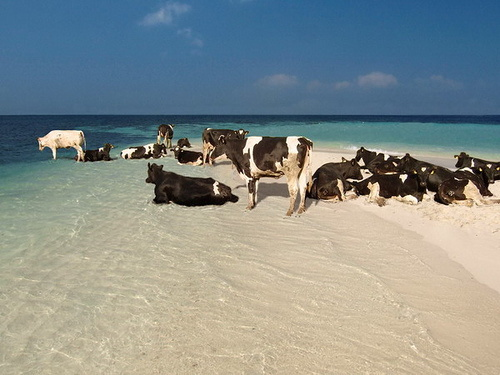
\includegraphics[scale=0.3]{Q3Images/cows_on_beach.jpg}
	\centerline{\small (1a) Imagem original}
\end{minipage}
\begin{minipage}[b]{0.45\textwidth}
	\centering
        
\includegraphics[scale=0.3]{Q3Images/cows_on_beach_ela.jpg} 
	\centerline{\small (1b) Imagem com o resultado do ELA}
\end{minipage}
\caption{Aplicação do método ELA}
\label{fig1}
\end{figure}

Os resultados foram avaliados de acordo com o brilho das bordas que devem ser semelhantes no resultado 
da aplicação do ELA na imagem. Além disso, regiões de cores e texturas semelhantes na imagem
original, independentemente da cor, também devem ter cores aproximadamente similares no ELA \cite{berkeleywebsite}.

Isto posto, considerei que um total de 23 imagens foram alteradas de acordo com o método e avaliação a posteriori. 
A Tabela \ref{table-hoax-imgs} lista a avaliação do método nas imagens dadas. As imagens originais, bem como as
alteradas pelo método podem ser vistas no diretório \textbf{source/HoaxImages}.
\begin{table}[]
\centering
\caption{Tabela com o resultado da aplicação do método ELA}
\label{table-hoax-imgs}
\begin{tabular}{|l|l|} \hline
Imagem                 & Alterada? \\ \hline
2000\_snowballcat.jpg  & Y         \\
bikefail.jpg           & N         \\
blacklion01.jpg        & Y         \\
bouncing\_baby.jpg     & N         \\
broken\_road.jpg       & N         \\
businahole.jpg         & N         \\
cows\_on\_beach.jpg    & Y         \\
cursor.jpg             & N         \\
daliatom.jpg           & Y         \\
dononwater.jpg         & N         \\
eagles.jpg             & N         \\
frozenvenice.jpg       & Y         \\
glass\_butterfly.jpg   & Y         \\
goldfish\_hitler.jpg   & N         \\
hatfield.jpg           & N         \\
hellephant.jpg         & N         \\
hitlerbaby.jpg         & N         \\
horseinahole01.jpg     & N         \\
houseboat01.jpg        & Y         \\
iceberg.jpg            & N         \\
jumping\_giraffe.jpg   & Y         \\
kissing.jpg            & Y         \\
koala01.jpg            & N         \\
leap.jpg               & Y         \\
magic\_tap.jpg         & Y         \\
manitoba\_security.jpg & Y         \\
moonmelon01.jpg        & Y         \\
nikolatesla.jpg        & Y         \\
queensguard.jpg        & N         \\
rainbow\_tornado.jpg   & N         \\
rocket\_bike.jpg       & Y         \\
sharkswim.jpg          & Y         \\
shark\_roof.jpg        & N         \\
skiing\_egypt.jpg      & Y         \\
skullrose.jpg          & N         \\
spacechair.jpg         & Y         \\
tandembike.jpg         & N         \\
tattooguy01.jpg        & y         \\
tennis.jpg             & Y         \\
tentacle\_bldg.jpg     & Y         \\
trafficlights.jpg      & N         \\
tunnelface01.jpg       & N         \\
verydeep.jpg           & N         \\
vuitton.jpg            & Y         \\
whale.jpg              & N         \\
wienerplane.jpg        & Y         \\ \hline
\end{tabular}
\end{table}

\end{itemize}
%
%
%
\item[{\bf Q2.}] Esta questão refere-se à transformada de Fourier.
\begin{itemize}
\item Encontre a transformada de Fourier da função:
\begin{eqnarray*}
f(x) = \left\{ \begin{array}{rl} 
 7 &\mbox{ if $-5 < x < 5$} \\
 0 &\mbox{ caso contrário}
       \end{array} \right.
\end{eqnarray*}

Por definição, temos que a transformada de Fourier de um pulso
retangular de duração $D$ e altura $A$ tem a forma dada por:

\begin{eqnarray*}
    F(\omega) = ADsinc\bigg(\frac{\omega D}{2}\bigg)  = AD\frac{sin(\frac{\omega D}{2})}{\frac{\omega D}{2}}
\end{eqnarray*}

A função $f(x)$ pode ser representada graficamente como (Figura \ref{fig:fig2}):
\begin{figure}[H]
    \centering
    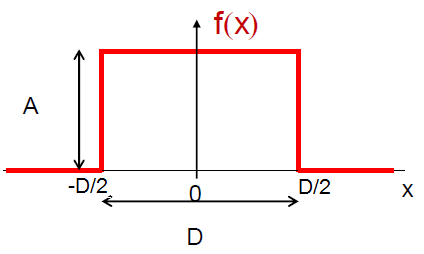
\includegraphics[width=0.3\textwidth]{Q3Images/pulse_function.png}
    \caption{Função pulso retangular}
    \label{fig:fig2}
\end{figure}

Onde:
\begin{eqnarray*}
f(x) = \left\{ \begin{array}{rl} 
 A, &\mbox{ $x \in  [\frac{-D}{2}, \frac{D}{2}]$} \\
 0, &\mbox{ $x \notin [\frac{-D}{2}, \frac{D}{2}]$}
       \end{array} \right.
\end{eqnarray*}

Logo, temos que A = 7 e D = 10 e, portanto, a transformada de Fourier da função $f(x)$ é:
\begin{align*}
    F(\omega) &= AD\frac{sin(\frac{\omega D}{2})}{\frac{\omega D}{2}} \\
              &= 7*10\frac{sin(\frac{\omega 10}{2})}{\frac{\omega 10}{2}} \\
              &= 70\frac{sin(\frac{\omega 10}{2})}{\frac{\omega 10}{2}} \\
              &= 70\frac{sin(5\omega)}{5\omega}
\end{align*}

%%%
\item Encontre a transformada de Fourier da função $ g(x) = f(x)\cos
   \omega_0 x$, sabendo que a transformada de Fourier de $f(x)$ é dada
   por $F(\omega)$

Tomando a propriedade da modulação:
\begin{align*}
    \mathcal{F}[x(t)cos(\omega_0t)] = \frac{1}{2}[F(\omega + \omega_0) + F(\omega - \omega_0)]
\end{align*}
Temos que a transformada de Fourier da função $g(x)$ é:
\begin{align*}
    G(\omega) = \frac{1}{2}F(\omega + \omega_0) + \frac{1}{2}F(\omega - \omega_0)
\end{align*}

%%%
\item Ache a inversa da transformada de Fourier de $G(\omega) =
  20\frac{\sin 5\omega}{5\omega}e^{-3\omega i}$

Por ora, ignorando a exponencial complexa de $G(\omega)$, podemos obter os valores de $A$ e $D$:
\begin{align*}
    20\frac{sin(5\omega)}{5\omega} = AD\frac{sin(\frac{\omega D}{2})}{\frac{\omega D}{2}} \\
    \\ 5\omega = \frac{\omega D}{2} \\
    10\omega = \omega D \\
    D = \frac{10\omega}{\omega} = 10 \\
    \\ AD = 20 \\
    A10 = 20 \\
    A = 2
\end{align*}

Tomando a representação da função $f(x)$ do pulso retangular de duração $D$ e amplitude $A$:
\begin{align*}
f(x) = A . rect(x) = \left\{ \begin{array}{rl}
 A, &\mbox{ $x \in  [\frac{-D}{2}, \frac{D}{2}]$} \\
 0, &\mbox{ $x \notin [\frac{-D}{2}, \frac{D}{2}]$}
       \end{array} \right.
\end{align*}

Vimos no primeiro item do exercício 2 que:
\begin{align*}
 A . rect\bigg(\frac{x}{D}\bigg) \xrightarrow{\mathscr{F}} ADsinc \bigg(\frac{\omega D}{2}\bigg)
\end{align*}

O que nos dá a forma do pulso retangular:
\begin{align*}
f(x) = 2 . rect\bigg(\frac{x}{10}\bigg) = \left\{ \begin{array}{rl} 
 2, &\mbox{ $x \in  [-5, 5]$} \\
 0, &\mbox{ $x \notin [-5, 5]$}
       \end{array} \right.
\end{align*}

Cuja representação gráfica é (Figura \ref{fig:fig3}):
\begin{figure}[H]
    \centering
    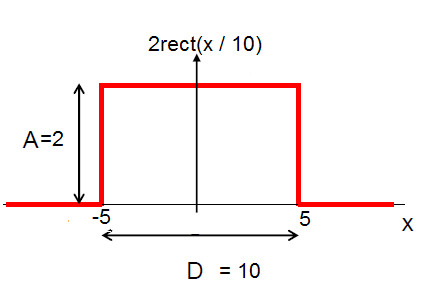
\includegraphics[width=0.3\textwidth]{Q3Images/pulse_function_2.png}
    \caption{Função pulso retangular com D = 10 e A = 2}
    \label{fig:fig3}
\end{figure}

Considerando agora a exponencial complexa, sabemos que ela representa um deslocamento no tempo,
que é $3$ neste caso e, portanto:
\begin{align*}
    2 . rect\bigg(\frac{x-3}{10}\bigg) \xrightarrow{\mathscr{F}} 20\frac{\sin 5\omega}{5\omega}e^{-3\omega i} \\
    g(x) = 2 . rect\bigg(\frac{x-3}{10}\bigg) = \left\{ \begin{array}{rl} 
     2, &\mbox{ $-2 < x < 8$} \\
     0, &\mbox{ caso contrário}
           \end{array} \right.
\end{align*}

\begin{figure}[H]
    \centering
    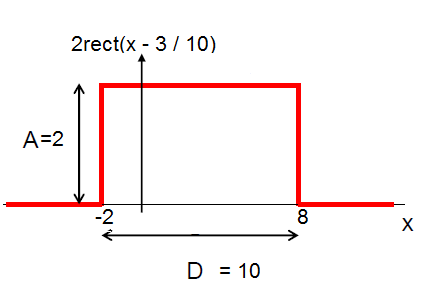
\includegraphics[width=0.3\textwidth]{Q3Images/pulse_function_3.png}
    \caption{Função pulso retangular com deslocamento no tempo}
    \label{fig:fig4}
\end{figure}

%%%
\item Calcule a DFT do sinal $f = \{1,3,5,3,1\}$

A Transformada Discreta de Fourier (DFT) provém da Série Discreta de Fourier (DFS) e é dada por \cite{broughton2009discrete}:
\begin{align*}
    X_k = \sum\limits_{m=0}^{N-1} x_m e^{\frac{-2\pi ikm}{N}},\qquad para\quad k=0,1,2,...,N-1
\end{align*}

Para realizar os cálculos devemos utilizar a identidade de Euler:
\begin{align*}
    e^{-i \pi} = \cos \pi - i\sin\pi
\end{align*}

Temos que N=5, ou seja, o tamanho do vetor do sinal dado por $f$, logo:
\begin{align*}
    &X_0 = (1e^0 + 3e^0 + 5e^0 + 3e^0 + 1e^0) &\\
    &X_1 = (1e^0 + 3e^{\frac{-2\pi i1}{5}} + 5e^{\frac{-2\pi i2}{5}} + 3e^{\frac{-2\pi i3}{5}} + 1e^{\frac{-2\pi i4}{5})} &\\
    &X_2 = (1e^0 + 3e^{\frac{-2\pi i2}{5}} + 5e^{\frac{-2\pi i4}{5}} + 3e^{\frac{-2\pi i6}{5}} + 1e^{\frac{-2\pi i8}{5})} &\\
    &X_3 = (1e^0 + 3e^{\frac{-2\pi i3}{5}} + 5e^{\frac{-2\pi i6}{5}} + 3e^{\frac{-2\pi i9}{5}} + 1e^{\frac{-2\pi i12}{5})} &\\
    &X_4 = (1e^0 + 3e^{\frac{-2\pi i4}{5}} + 5e^{\frac{-2\pi i8}{5}} + 3e^{\frac{-2\pi i12}{5}} + 1e^{\frac{-2\pi i16}{5})} &\\
    \\&X_0 = (1 + 3 + 5 + 3 + 1) &\\
    &X_1 = (1 + 3e^{\frac{-2\pi i}{5}} + 5e^{\frac{-4\pi i}{5}}  + 3e^{\frac{-6\pi i}{5}}  + 1e^{\frac{-8\pi i}{5})} &\\
    &X_2 = (1 + 3e^{\frac{-4\pi i}{5}} + 5e^{\frac{-8\pi i}{5}}  + 3e^{\frac{-12\pi i}{5}} + 1e^{\frac{-16\pi i}{5})} &\\
    &X_3 = (1 + 3e^{\frac{-6\pi i}{5}} + 5e^{\frac{-12\pi i}{5}} + 3e^{\frac{-18\pi i}{5}} + 1e^{\frac{-24\pi i}{5})} &\\
    &X_4 = (1 + 3e^{\frac{-8\pi i}{5}} + 5e^{\frac{-16\pi i}{5}} + 3e^{\frac{-24\pi i}{5}} + 1e^{\frac{-32\pi i}{5})}&
\end{align*}
Calculando cada exponencial complexa com a relação de Euler e substituindo os resultados na equação acima:
\begin{align*}
    &e^{\frac{-2\pi i}{5}} = cos(\frac{2\pi}{5}) - isen(\frac{2\pi}{5}) = 0.30902  - 0.95106i &\\
    &e^{\frac{-4\pi i}{5}} = cos(\frac{4\pi}{5}) - isen(\frac{4\pi}{5}) = -0.80902 - 0.58779i &\\
    &e^{\frac{-6\pi i}{5}} = cos(\frac{6\pi}{5}) - isen(\frac{6\pi}{5}) = -0.80902 + 0.58779i &\\
    &e^{\frac{-8\pi i}{5}} = cos(\frac{8\pi}{5}) - isen(\frac{8\pi}{5}) = 0.30902  - 0.95106i &\\
    &e^{\frac{-12\pi i}{5}} = cos(\frac{12\pi}{5}) - isen(\frac{12\pi}{5}) = 0.30902	-0.95106i &\\
    &e^{\frac{-16\pi i}{5}} = cos(\frac{16\pi}{5}) - isen(\frac{16\pi}{5}) = -0.80902 + 0.58779i &\\
    &e^{\frac{-18\pi i}{5}} = cos(\frac{18\pi}{5}) - isen(\frac{18\pi}{5}) = 0.30902 + 0.95106i &\\
    &e^{\frac{-24\pi i}{5}} = cos(\frac{24\pi}{5}) - isen(\frac{24\pi}{5}) = -0.80902 - 0.58779i &\\
    &e^{\frac{-32\pi i}{5}} = cos(\frac{32\pi}{5}) - isen(\frac{32\pi}{5}) = 0.30902	- 0.95106i&
\end{align*}

Temos então que o resultado da DFT é:
\begin{multline*}
    X[x] = 13.0, -4.236067-3.077683i, 0.236067+0.726542i, \\
           0.236067-0.726542i, -4.236067+3.077683i
\end{multline*}

\end{itemize}
%
%
%
\item[{\bf Q3.}]
\begin{itemize}
\item Calcule (apresente os cálculos) dos descritores de Fourier das
  figuras 5a e 5b. Lembre-se que os pontos da
  borda do quadrado serão representados por pontos no plano de
  Argand-Gauss. Isto é, cada ponto no plano passa a ser um número
  complexo e a borda passa a ser um vetor de pontos complexos, como
  num sinal, mas com valores complexos.

\begin{figure}[htb]
    \centering
    \begin{minipage}[b]{0.45\textwidth}
    	\centering
            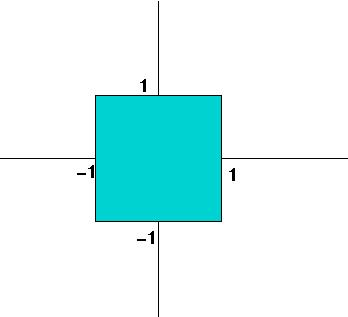
\includegraphics[scale=0.2]{Q3Images/square1.jpg} 
    	\centerline{\small (5a) Quadrado de lado 1}
    \end{minipage}
    \begin{minipage}[b]{0.45\textwidth}
    	\centering
            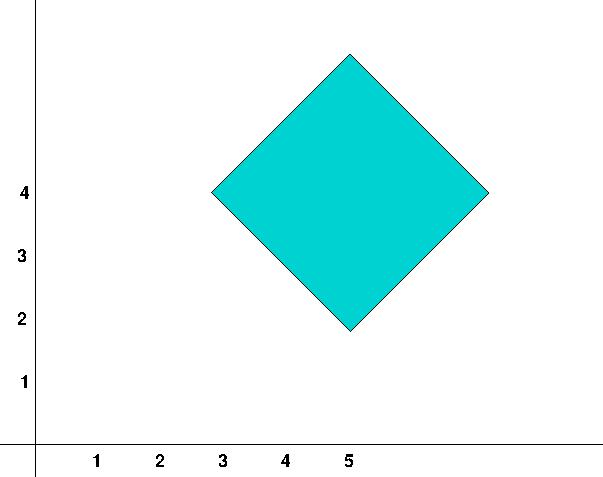
\includegraphics[scale=0.3]{Q3Images/square3.jpg} 
    	\centerline{\small (5b) Quadrado de lado 3}
    \end{minipage}
\caption{Figuras no plano cartesiano}
\label{fig:fig5}
\end{figure}

\textbf{Resultados para a primeira imagem}

Para que possamos calcular os descritores de Fourier, devemos representar as coordenadas do quadrado (1,1), (-1,1), (-1,-1) e (1,-1), como 
coordenadas no plano de Argand-Gauss que, neste caso, são: (1 + i, -1 + i, -1 - i, 1 - i).

Os descritores de Fourier podem ser calculados a partir da DFT \cite{broughton2009discrete}:
\begin{align*}
    X_k = \sum\limits_{m=0}^{N-1} x_m e^{\frac{-2\pi ikm}{N}},\qquad para\quad k=0,1,2,...,N-1
\end{align*}

Da mesma forma que no item anterior, para realizar os cálculos devemos utilizar a identidade de Euler:
\begin{align*}
    e^{-i \pi} = \cos \pi - i\sin\pi
\end{align*}
	  
Temos que N=4, ou seja, o número de pontos no plano de Argand-Gauss, logo:
\begin{align*}
    &X_0 = (1 + i)e^0 + (-1 + i)e^0 + (-1 - i)e^0 + (1 - i)e^0 &\\
    &X_1 = (1 + i)e^0 + (-1 + i)e^{\frac{-2\pi i1}{4}} + (-1 - i)e^{\frac{-2\pi i2}{4}} + (1 - i)e^{\frac{-2\pi i3}{4}} &\\
    &X_2 = (1 + i)e^0 + (-1 + i)e^{\frac{-2\pi i2}{4}} + (-1 - i)e^{\frac{-2\pi i4}{4}} + (1 - i)e^{\frac{-2\pi i6}{4}} &\\
    &X_3 = (1 + i)e^0 + (-1 + i)e^{\frac{-2\pi i3}{4}} + (-1 - i)e^{\frac{-2\pi i6}{4}} + (1 - i)e^{\frac{-2\pi i9}{4}} &\\
    \\
    &X_0 = (1 + i) + (-1 + i) + (-1 - i) + (1 - i)) &\\
    &X_1 = (1 + i) + (-1 + i)e^{\frac{-2\pi i}{4}} + (-1 - i)e^{\frac{-4\pi i}{4}} + (1 - i)e^{\frac{-6\pi i}{4}} &\\
    &X_2 = (1 + i) + (-1 + i)e^{\frac{-4\pi i}{4}} + (-1 - i)e^{\frac{-8\pi i}{4}} + (1 - i)e^{\frac{-12\pi i}{4}} &\\
    &X_3 = (1 + i) + (-1 + i)e^{\frac{-6\pi i}{4}} + (-1 - i)e^{\frac{-12\pi i}{4}} + (1 - i)e^{\frac{-18\pi i}{4}} &
\end{align*}

Calculando cada exponencial complexa com a relação de Euler e substituindo os resultados na equação acima:
\begin{align*}
    &e^{\frac{-2\pi i}{4}} = cos(\frac{2\pi}{4}) - isen(\frac{2\pi}{4}) = -i &\\
    &e^{\frac{-4\pi i}{4}} = cos(\frac{4\pi}{4}) - isen(\frac{4\pi}{4}) = -1 &\\
    &e^{\frac{-6\pi i}{4}} = cos(\frac{6\pi}{4}) - isen(\frac{6\pi}{4}) = i &\\
    &e^{\frac{-8\pi i}{4}} = cos(\frac{8\pi}{4}) - isen(\frac{8\pi}{4}) = 1 &\\
    &e^{\frac{-12\pi i}{4}} = cos(\frac{12\pi}{4}) - isen(\frac{12\pi}{4}) = -1 &\\
    &e^{\frac{-18\pi i}{4}} = cos(\frac{18\pi}{4}) - isen(\frac{18\pi}{4}) = -i &
\end{align*}
Temos então que o resultado dos descritores de Fourier da imagem é:
\begin{align*}
    &X_0 = 0 &\\
    &X_1 = (1 + i) + (-1 + i)*(-i) + (-1 - i)*(-1) + (1 - i)*(i) &\\
    &X_2 = (1 + i) + (-1 + i)*(-1) + (-1 - i)*(1) + (1 - i)*(-1) &\\
    &X_3 = (1 + i) + (-1 + i)*(i) + (-1 - i)*(-1) + (1 - i)*(-i) &\\
    \\
    &X[x] = 0.0, 4 + 4i, 0.0, 0.0 &
\end{align*}

\textbf{Resultados para a segunda imagem}

Assim como fizemos no item anterior, devemos calcular as coordenadas da imagem para encontrarmos os descritores de Fourier.
Sabemos a coordenada x dos pontos inferior e superior do quadrilátero, que é 5 e, também, conhecemos a coordenada do eixo y para os ponto mais à esquerda e à direita que é igual a 4.

Para as demais coordenadas, basta calcular o valor da diagonal do quadrilátero que, neste caso, é a hipotenusa dos dois triângulos retângulos formados ao se dividir o quadrilátero ao meio, cujos lados possuem comprimento 3. 
    
Com base no teorema de Pitágoras temos que a hipotenusa c desse triângulo é dado por:
\begin{align*}
 c^2 &= a^2 + b^2 \\
 c^2 &= 3^2 + 3^2 \\
 c &= \sqrt{18}	     
\end{align*}

Consequentemente, temos que a diagonal é $d = \sqrt{18} = 4.24264$ e as coordenadas dos pontos da imagem, que denominei de $f$, são:
\begin{align*}
    f &= (5, 4 + \frac{4.24264}{2}), (5 - \frac{4.24264}{2}, 4), (5, 4 - \frac{4.24264}{2}), (5 + \frac{4.24264}{2}, 4) \\
    f &= (5, 6.12132), (2.87868, 4), (5, 1.87868), (7.12132, 4)
\end{align*}
    
Agora, devemos representar as coordenadas por pontos no Plano de Argand-Gauss, que são:
\begin{align*}
    f &= (5 + 6.12132i, 2.87868 + 4i, 5 + 1.87868i, 7.12132 + 4i)
\end{align*}

Os descritores de Fourier podem ser calculados a partir da DFT \cite{broughton2009discrete}:
\begin{align*}
    X_k = \sum\limits_{m=0}^{N-1} x_m e^{\frac{-2\pi ikm}{N}},\qquad para\quad k=0,1,2,...,N-1
\end{align*}

Novamente, utilizando a identidade de Euler:
\begin{align*}
    e^{-i \pi} = \cos \pi - i\sin\pi
\end{align*}
	  
Temos que N=4, ou seja, o número de pontos no plano de Argand-Gauss, logo:
\begin{align*}
    &X_0 = (5 + 6.12132i)e^0 + (2.87868 + 4i)e^0 + (5 + 1.87868i)e^0 + (7.12132 + 4i)e^0 &\\
    &X_1 = (5 + 6.12132i)e^0 + (2.87868 + 4i)e^{\frac{-2\pi i1}{4}} + (5 + 1.87868i)e^{\frac{-2\pi i2}{4}} + (7.12132 + 4i)e^{\frac{-2\pi i3}{4}} &\\
    &X_2 = (5 + 6.12132i)e^0 + (2.87868 + 4i)e^{\frac{-2\pi i2}{4}} + (5 + 1.87868i)e^{\frac{-2\pi i4}{4}} + (7.12132 + 4i)e^{\frac{-2\pi i6}{4}} &\\
    &X_3 = (5 + 6.12132i)e^0 + (2.87868 + 4i)e^{\frac{-2\pi i3}{4}} + (5 + 1.87868i)e^{\frac{-2\pi i6}{4}} + (7.12132 + 4i)e^{\frac{-2\pi i9}{4}} &\\
    \\
    &X_0 = (5 + 6.12132i) + (2.87868 + 4i) + (5 + 1.87868i) + (7.12132 + 4i)) &\\
    &X_1 = (5 + 6.12132i) + (2.87868 + 4i)e^{\frac{-2\pi i}{4}} + (5 + 1.87868i)e^{\frac{-4\pi i}{4}} + (7.12132 + 4i)e^{\frac{-6\pi i}{4}} &\\
    &X_2 = (5 + 6.12132i) + (2.87868 + 4i)e^{\frac{-4\pi i}{4}} + (5 + 1.87868i)e^{\frac{-8\pi i}{4}} + (7.12132 + 4i)e^{\frac{-12\pi i}{4}} &\\
    &X_3 = (5 + 6.12132i) + (2.87868 + 4i)e^{\frac{-6\pi i}{4}} + (5 + 1.87868i)e^{\frac{-12\pi i}{4}} + (7.12132 + 4i)e^{\frac{-18\pi i}{4}} &
\end{align*}

Calculando cada exponencial complexa com a relação de Euler e substituindo os resultados na equação acima:
\begin{align*}
    &e^{\frac{-2\pi i}{4}} = cos(\frac{2\pi}{4}) - isen(\frac{2\pi}{4}) = -i &\\
    &e^{\frac{-4\pi i}{4}} = cos(\frac{4\pi}{4}) - isen(\frac{4\pi}{4}) = -1 &\\
    &e^{\frac{-6\pi i}{4}} = cos(\frac{6\pi}{4}) - isen(\frac{6\pi}{4}) = i &\\
    &e^{\frac{-8\pi i}{4}} = cos(\frac{8\pi}{4}) - isen(\frac{8\pi}{4}) = 1 &\\
    &e^{\frac{-12\pi i}{4}} = cos(\frac{12\pi}{4}) - isen(\frac{12\pi}{4}) = -1 &\\
    &e^{\frac{-18\pi i}{4}} = cos(\frac{18\pi}{4}) - isen(\frac{18\pi}{4}) = -i &
\end{align*}
Temos então que o resultado dos descritores de Fourier da imagem é:
\begin{align*}
    &X_0 = (5 + 6.12132i) + (2.87868 + 4i) + (5 + 1.87868i) + (7.12132 + 4i) &\\
    &X_1 = (5 + 6.12132i) + (2.87868 + 4i)*(-i) + (5 + 1.87868i)*(-1) + (7.12132 + 4i)*(i) &\\
    &X_2 = (5 + 6.12132i) + (2.87868 + 4i)*(-1) + (5 + 1.87868i)*(1) + (7.12132 + 4i)*(-1) &\\
    &X_3 = (5 + 6.12132i) + (2.87868 + 4i)*(i) + (5 + 1.87868i)(-1) + (7.12132 + 4i)*(-i) &\\
    \\
    &X[x] = 20.0 + 16i,  8.428528i, 0.0, 0.0&
\end{align*}
     
\item Para confirmar que seus cálculos estão corretos, implemente um
  programa em Python que receba como entrada um vetor de números
  complexos (que são as coordenadas das bordas) e retorne os
  descritores de Fourier do vetor de entrada. Você pode usar as
  funções fornecidas pela biblioteca NUMPY para facilitar a
  programação.
  
O programa foi implementado em Python, com a biblioteca Numpy e está localizado em \textbf{source/fourier\_descriptors.py}.\\

\item Para reconstruir a curva, faça uma função que receba um vetor
  com os descritores de Fourier, um número $N$ de descritores a serem
  usados e grafique os pontos num plano cartesiano (para fazer a mesma 
figura que fizemos nos slides das aulas 15 e 16.

O programa foi implementado em Python, com a biblioteca Numpy e está localizado em \textbf{source/ifd.py}.\\
Basta executar o arquivo e passar um array com os descritores para que os pontos sejam desenhados. O tamanho
$N$ do vetor é calculado pelo programa.\\
A Figura \ref{fig:fig6}, por exemplo, foi gerada com o vetor de entrada:
\\$0+4j, 2+4j, 3+3j, 3+2j, 2+1j, 2-1j, 1-2j, 0-3j,-1-3j, -2-2j, -2+0j, -2+1j, -1+3j$

\begin{figure}[H]
    \centering
    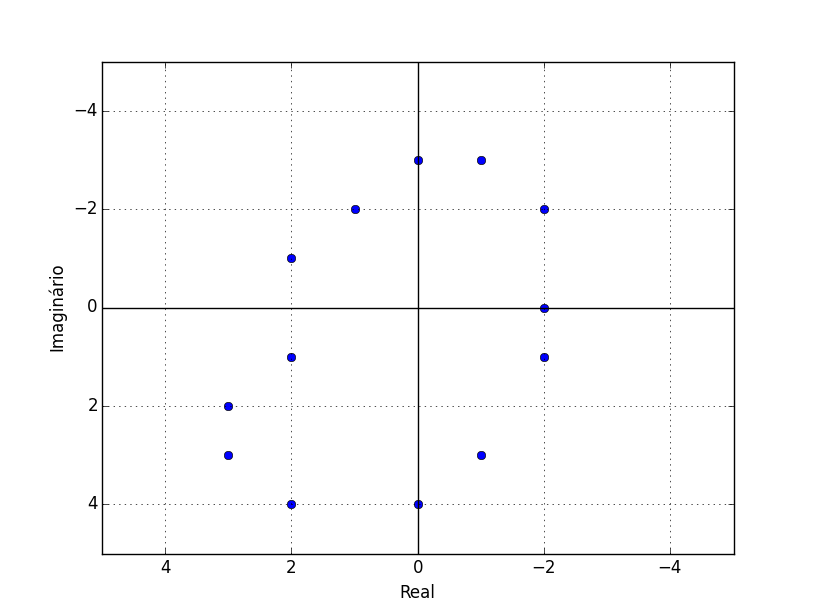
\includegraphics[width=0.5\textwidth]{Q3Images/fdescriptors_points.png}
    \caption{Exemplo de pontos de contorno a partir de descritores de Fourier}
    \label{fig:fig6}
\end{figure}

\end{itemize}
%
%
%
\item[{\bf Q4.}] \textbf{Apenas para os alunos de pós-graduação}
\begin{itemize}
\item Leia o artigo do Torre e do Poggio
  \url{ftp://publications.ai.mit.edu/ai-publications/pdf/AIM-768.pdf}
  e faça um resumo de acordo com as indicações que deixei no
  paca (artigos sobre como fazer um resumo). 

  \noindent\rule{14.5cm}{0.4pt}

\begin{center}
    {\Large Resumo: \textit{On Edge Detection}}
    \\[8pt]
    
    \textit{Rodrigo Augusto Dias Faria}
    \\[8pt]
    
    \textit{Instituto de Matemática e Estatística -- Universidade de São Paulo (IME-USP)\\
    Departamento de Ciência da Computação
    }\\[8pt]
    
    \texttt{rofaria@ime.usp.br, rodrigoadfaria@gmail.com}
\end{center}

\begin{enumerate}
\item \textbf{Resumo}
\begin{enumerate}[label*=\arabic*.]
    \item \textbf{Motivação}
    
    \textbf{What is the research problem the paper attempts to address?}\\
    Uma borda em uma imagem é caracterizada por um conjunto de pixels conectados que ficam na fronteira entre duas regiões de uma imagem com propriedades relativamente distintas de nível de cinza \cite{gonzalez2002digital}. Em outras palavras, as bordas caracterizam-se por mudanças na intensidade da imagem em termos de aspectos físicos que as originaram \cite{Torre-1986}.
    
    Em processamento de imagens, a percepção da mudança de intensidade pode ser obtida por vários métodos que, em geral, utilizam de um operador local diferencial para delinear as bordas.
    
    Torre e Poggio subdividem a detecção de bordas em duas etapas: uma etapa de filtragem para eliminação de ruídos da imagem  e uma segunda etapa que caracteriza-se pela avaliação das derivadas da intensidade da imagem, sendo esta última classificada como um problema de diferenciação numérica.
    
    Sabendo que a diferenciação numérica não é robusta contra ruído, Torre e Poggio mostram que a diferenciação de uma função $f(x)$ é um típico problema mal-posto e pode ser visto como a solução do problema inverso
\begin{equation} \label{eq:inverse_problem}
   g(x) = A f(x)
\end{equation}

onde $A f(x)$ é o operador integral

\begin{equation} \label{eq:inverse_int}
   \int_{-\infty}^{x} f(\tilde{x}) d\tilde{x} = \int_{-\infty}^{\infty} h(x - \tilde{x}) f(\tilde{x}) d\tilde{x}
\end{equation}

e $h$ é a função degrau.
    
    \textbf{What is the motivation of the research work?}\\
    Uma vez que a diferenciação numérica é um problema mal-posto no sentido de Hadamard, conforme mostrado pelos autores, a motivação dá-se, então, em regularizar o problema para que ele se torne bem-posto por meio de uma operação de filtragem antes da diferenciação.
    
    \textbf{Is there a crisis in the research field that the paper attempts to resolve?}\\
    Pode-se dizer que não há nenhuma crise evidente na área pesquisada pelos autores, mas
    
    \textbf{Is the research work attempting to overcome the weaknesses of existing approaches?}\\
    há demonstrações de que a proposta de realizar uma operação de filtragem antes da diferenciação, reduz a sensibilidade a ruído a que esta etapa está suscetível, algo não considerado por alguns métodos, tais como o proposto por Shanmugam, Dickey e Green que não faz nenhuma referência explícita à etapa de diferenciação.
    Vale ressaltar que, mesmo uma pequena quantidade de ruído na imagem produz um efeito crítico na diferenciação causando perturbação nos dados.
    
    \textbf{In short, what is the niche of the paper?}\\
    Em suma, Torre e Poggio deixam claro que para tornar o problema de diferenciação bem-posto é necessário que as intensidades da imagem sejam regularizadas, cujo processo pode ser feito por uma operação de filtragem antes da diferenciação e, para tal, eles estudaram propriedades de diferentes tipos de filtros, bem como a relação entre vários operadores diferenciais bidimensionais. Além disso, propriedades geométricas e topológicas desses operadores também são avaliadas com o objetivo de obter bordas mais suaves, dentre outras características interessantes.
    \\[6pt]

    \item \textbf{Contribuição}
    
    \textbf{What are the claimed contributions of the paper?}\\
    Os autores também mostram que há três métodos principais de regularização de acordo com a definição de Bertero. Além disso, a diferenciação também pode ser regularizada com operadores de estabilização de Tikhonov, que neste caso são equivalentes a filtragem dos dados com filtros passa-baixa.\\
    Com o intuito de reformular os resultados obtidos por Schoenberg, Poggio, Voorhees e Yuille \cite{Poggio1988106}, em um trabalho que, à época, ainda não havia sido publicado, provaram que a solução para a regularização do problema da diferenciação numérica em dados não exatos, pode ser obtida pela convolução dos dados com um filtro, que neste caso é uma spline cúbica, que por sua vez, é muito similar à uma Gaussiana.
    
    \textbf{What is new in this paper?}\\
    O resultado obtido por Poggio, citado em forma de teorema neste trabalho, é a prova mais simples e rigorosa de que um filtro Gaussiano representa a correta operação a ser realizada antes da diferenciação para detecção de borda.\\
    Esta justificativa dá o potencial de inovação e importante contribuição para mostrar que a filtragem seguida pela diferenciação podiam ser reconhecidas como operações presentes na maioria dos métodos de detecção de borda existentes até então.
    
    \textbf{A new proof technique? A new formalism or notation?}\\
    Vale ressaltar ainda que Poggio \cite{Poggio1988106} analisa o papel do parâmetro de regularização $\lambda$, sua conexão com a escala do filtro Gaussiano e discute métodos para encontrar o parâmetro $\lambda$ ótimo.
    
    Outra contribuição importante feita por Torre e Poggio foi a observação de três tipos de filtros: passa banda, suporte limitado e de incerteza mínima, sendo que o filtro passa banda, bem como de incerteza mínima são bons operadores de regularização para a diferenciação no sentido de Tikhonov.
    \textbf{In short, what is innovative about this paper?}
    \\[6pt]

    \item \textbf{Metodologia}
    
    \textbf{How do the authors substantiate their claims?}\\
    Os autores fundamentam o trabalho, a princípio, postando a natureza do problema de diferenciação numérica como um problema mal-posto de encontrar $x$ dos dados $y$ tal que $Az = y$, sendo que para a regularização é necessário a escolha de normas adequadas $||.||$ e de um funcional de estabilização $||Pz||$.\\
    Logo, três métodos de regularização propostos por Bertero são mostrados. O primeiro consiste em encontrar a função $z$ que minimiza $||Az - y||$ e satisfaz a restrição $||Pz|| < C_{1}$, onde $C_{1}$ é uma constante.\\
    O segundo calcula a função $z$ que está suficientemente próxima dos dados e é mais regular, minimizando $||Pz||$ e obedecendo à restrição $||Az - y|| \leq C_{2}$, onde $C_{2}$ é uma constante.\\
    O último método consiste em encontrar a função $z$ que minimiza $||Az - y||^2 + \lambda ||Pz||^2$, onde $\lambda$ é um parâmetro de regularização que controla o grau de regularização da solução e a aproximação dos dados.\\
    Outra forma de regularizar o problema de diferenciação são os operadores de Tikhonov que são equivalentes à filtragem dos dados com filtros passa-baixa.\\
    
    \textbf{What are the major theorems?}\\
    Conforme supra citado, Poggio \textit{et al.} \cite{Poggio1988106} reformulou os resultados obtidos por Schoenberg, na forma de um teorema que diz que a interpolação de uma spline cúbica em uma estrutura regular, satisfazendo o segundo método de regularização com $P = d^2 / dx^2$, pode ser obtida pela convolução dos dados com um filtro spline cúbico, que é uma função $L^4$ de Schoenberg, onde $P$ corresponde a forma mais simples do funcional de Tikhonov. Logo, a regularização pode ser obtida realizando a convolução dos dados com a primeira derivada do filtro $L^4$ de Shoenberg.\\
    No caso de dados não exatos, Poggio \textit{et al.} \cite{Poggio1988106} utilizou o terceiro método de regularização que, por conseguinte, originou um novo teorema proposto neste artigo provando que a solução pode ser obtida pela convolução dos dados com um filtro, o qual é uma spline cúbica e é muito similar a uma Gaussiana.\\
    Essa implicação é determinante para demonstrar que a convolução dos dados pode, então, ser realizada com um filtro Gaussiano.\\
    Tão logo, Torre e Poggio avaliam três tipos de filtros que podem ser utilizados nessa etapa, observando o tipo da derivada, se direcionais ou invariantes à rotação, e o tipo de representação, se zeros ou extremos. Os filtros de banda limitada satisfazem todas as condições de Tikhonov para a regularização da diferenciação, bem como os filtros de incerteza mínima.\\
    Já o caso dos filtros de suporte limitado, os autores mostram que o \textit{blurring} é uma classe desse tipo de filtro que falha em atender algumas propriedades para que possa ser aplicado à convolução. Em particular, a condição $\tilde{F}(\omega, \alpha) j\omega$ pertence a $L_{2}(-\infty, \infty)$, não é satisfeita, uma vez que a diferenciação introduz de volta altas frequências na mesma quantidade em que elas foram removidas por este tipo de filtragem.\\
    Vale lembrar que, a função Gaussiana $e^{-x^2/\sigma^2}$ é a função real $f \in L^2$ que minimiza a incerteza definida por $\Delta U = \Omega X$ no domínio da frequência e do espaço e, por essa razão, foi escolhida como o filtro ótimo por Marr e Hildreth na elaboração do trabalho que originou o operador Laplaciano do Gaussiano.\\
    
    \textbf{What experiments are conducted?}\\
    Torre e Poggio fazem ainda uma comparação entre a função prolato e a Gaussiana, com o objetivo de mostrar uma aproximação satisfatória entre ambas, de acordo com parâmetros pré definidos. Além disso, eles mostram a robustez das propriedades de regularização do filtro Gaussiano, comparando a convolução do mesmo com uma imagem $I(x, y)$ vista como a solução da equação do calor no caso bidimensional.\\
    Tendo devidamente estudado a etapa de regularização e filtragem, a etapa de diferenciação foi dividida nos operados diferenciais direcionais e os operados diferenciais invariantes à rotação.\\
    O primeiro provoca manchas nos contornos com passagens em zero, mas não pelo uso do operador e sim pela distorção introduzida por um operador de largura demasiada.\\
    No caso dos operadores invariantes à rotação, dois deles merecem destaque por serem amplamente utilizados em função de possuírem características interessantes que são o Laplaciano $\nabla ^2$, que é um operador linear e a derivada segunda ao longo do gradiente $\frac{\partial^2}{\partial n^2}$, que é um operador não linear.
    
    
    \textbf{Data analyses?}\\
    \textbf{Simulations?\\ Benchmarks?}\\
    \textbf{User studies?}\\
    \textbf{Case studies?}\\
    \textbf{Examples?}\\
    \textbf{In short, what makes the claims scientific (as opposed to being mere opinions1)?}
    \\[6pt]

    \item \textbf{Conclusão}
    
    \textbf{What are the conclusions?}\\
    \textbf{What have we learned from the paper?}\\
    \textbf{Shall the standard practice of the field be changed as a result of the new findings?}\\
    \textbf{Is the result generalizable?}\\
    \textbf{Can the result be applied to other areas of the field?}\\
    \textbf{What are the open problems?}\\
    \textbf{In short, what are the lessons one can learn from the paper?}

\end{enumerate}
\end{enumerate}

\noindent\rule{14.5cm}{0.4pt}
  \clearpage

\item O que é um problema mal-posto?
\\Um problema matemático é bem-posto, de acordo com a definição de Hadamard, se ele cumpre as seguintes condições:
\begin{enumerate}
  \item Existe solução;
  \item A solução é única;
  \item A solução tem uma dependência contínua com os dados de entrada (quando o problema não é somente bem-posto, 
  mas também, bem-condicionado, portanto, é robusto contra ruído);
\end{enumerate}  

Logo, um problema é dito mal-posto se alguma das condições acima não é satisfeita.  
\\No artigo em questão, o problema mal-posto trata-se da diferenciação de uma função $f(x)$ que é um típico problema mal-posto e pode ser visto como a solução do problema inverso visto no resumo em (\ref{eq:inverse_problem}) e (\ref{eq:inverse_int}).\\

\item O que é regularização?
\\Regularização, em linhas gerais, é a aproximação de um problema mal-posto por uma família de problemas bem-postos \cite{Engl-1981}.
\\Conforme visto no item anterior, como temos um problema de diferenciação numérica e é sabido que ele é mal-posto, os autores 
avaliaram alguns métodos de regularização para, então, aproximar uma solução.
\\Um dos possíveis métodos são os operadores de Tikhonov que, para equações de convolução como em (\ref{eq:inverse_int}),
os operadores correspondem à convolução de $g(x)$ com um filtro $F(x, \alpha)$, onde $\alpha$ é um parâmetro.\\

\item Qual a importância do teorema apresentado no artigo?
\\No caso de dados não exatos, Poggio \textit{et al.} \cite{Poggio1988106} utilizou o terceiro método de regularização proposto por Bertero que, por conseguinte, originou um novo teorema proposto por Torre e Poggio provando que a solução para o problema de diferenciação pode ser obtida pela convolução dos dados com um filtro, o qual é uma spline cúbica e é muito similar a uma Gaussiana.\\
    Essa implicação é determinante para demonstrar que a convolução dos dados pode, então, ser realizada com um filtro Gaussiano.\\

\item O que são filtros de banda limitada? Qual a sua importância no artigo?
\textbf{TODO}\\

\item Quais são os métodos de encontrar borda apresentados no artigo?
\\Os métodos de detecção de borda apresentados no artigo são:
\begin{enumerate}[label*=\arabic*.]
    \item \textbf{Difference of Boxes - DOB}\\
    Proposto por Herskovitz e Binford, o filtro DOB é do tipo suporte limitado e utiliza a função de Haar para filtragem direcional
    ou diferença de funções para filtragem rotacional.
    A função de Haar tem a propriedade de ser um filtro ótimo de suporte limitado que maximiza a relação sinal-ruído.
    \\
    \item \textbf{Shanmugam, Dickey and Green}\\
    O operador proposto por Shanmugam, Dickey e Green, como citado por Torre e Poggio, é um filtro ótimo na medida em que produz o máximo de energia dentro de um intervalo de um dado espaço ao redor da borda. Eles analisaram os casos contínuo e discreto e concluíram que a implementação pode ser realizada por meio da Transformada Rápida de Fourier (FFT).
    \\
    \item \textbf{Laplacian of Gaussian - LOG}\\
    Proposto por Marr e Hildreth, o Laplaciano do Gaussiano combina a filtragem Gaussiana para a suavização da imagem, com o operador Laplaciano
    que localiza as bordas pela presença de um cruzamento em zero na derivada segunda com um pico acentuado correspondente à derivada primeira \cite{pedrini2008analise}.\\
    A saída do operador é dada pela operação de convolução
    \begin{equation} \label{eq:log}
        (\nabla^2 G(x, y)) * f(x, y)
    \end{equation}
    onde $f(x, y)$ é uma imagem suavizada por uma função Gaussiana.
    \\
    \item \textbf{Haralick}\\
    O método proposto por Haralick consiste em marcar um pixel como parte integrante da borda se na sua vizinhança há passagens em zero da segunda derivada ao longo do gradiente. Com o propósito de calcular as derivadas, Haralick aproxima e interpola os valores de intensidade amostrados com polinômios discretos de Chebychev.
    \\
    \item \textbf{Canny}\\
    De acordo com Pedrini \cite{pedrini2008analise}, com o intuito de otimizar a localização de pontos de borda na presença de ruído, o método de Canny suaviza a imagem por meio de um filtro Gaussiano e, em seguida, a magnitude e a direção do gradiente são calculadas utilizando aproximações baseadas em diferenças finitas para as derivadas parciais.\\
    Após o cálculo do gradiente, a borda é localizada utilizando supressão não-máxima, ou seja, apenas os pontos cuja magnitude seja localmente máxima na direção do gradiente.\\
    Fragmentos espúrios causados pela presença de ruído ou textura fina são então removidos com a aplicação de dois limiares diferentes, cujo processo é conhecido como \textit{limiarização por histerese}.
    \\
\end{enumerate}

\end{itemize}
\end{itemize}
\clearpage

\printbibliography
\end{document}